%%%%%%%%%%%%%%%%%%%%%%%%%%%%%%%%%%%%%%%%%%%%%%%%%%%%%%%%%%%%%%%%%%%%%%%%%%%%%%%%%%
%%																				%%
%% File name: 		00sarah.tex													%%
%% Project name:	Hochleistungsantenne										%%
%% Type of work:	T3X00 project work											%%
%% Author:			Sarah Brückner, Maximilian Stiefel, Hannes Bohnengel		%%
%% Date:			27th Arpil 2016												%%
%% University:		DHBW Ravensburg Campus Friedrichshafen						%%
%% Comments:		Created in gedit with tab width = 4							%%
%%																				%%
%%%%%%%%%%%%%%%%%%%%%%%%%%%%%%%%%%%%%%%%%%%%%%%%%%%%%%%%%%%%%%%%%%%%%%%%%%%%%%%%%%
%\cite{kauffels}\newpar

\chapter{Projektmanagement}
Schon Thomas Carlyle (1795–1881) erkannte die Wichtigkeit von strukturierten und organisiertem Vorgehen als er sagte:\newpar
``Unsere Hauptaufgabe ist nicht, zu erkennen, was unklar in weiter Entfernung liegt, sondern zu tun, was klar vor uns liegt''.\newpar
In einem Projekt ist das strukturierte und ogranisierte Vorgehen der klare Weg zu einem erfolgreichem Ziel. Daher wird sich in dieser Arbeit
dem Projektmanagement bedient um die Antennennachführung für Satelliten in die richtige Richtung zu lotzen. Dabei lehnt sich das Management an 
das V-Modell, welche den Abflauf von Software-, als auch von Hardwareentwicklungsprozessen beschreibt. Dieses Modell soll einem Projekt 
die Richtung weisen, jedoch werden die einzelnen Schritte vom Projektmanager selbst definiert. Ein Vorgehensmodell wie dieses legt folgende
Prozesse fest:
\begin{itemize}
 \item die Aktivitäten die durchzuführen sind,
 \item die Reihenfolge des Arbeitsablaufes,
 \item die Definition von Ergebnissen,
 \item die Fertigstellungskriterien,
 \item die Ressourcen die vorhanden sind
 \item und die anzuwendenden Standards/Werkzeuge.
\end{itemize}
\begin{figure}[h]
 \centering
 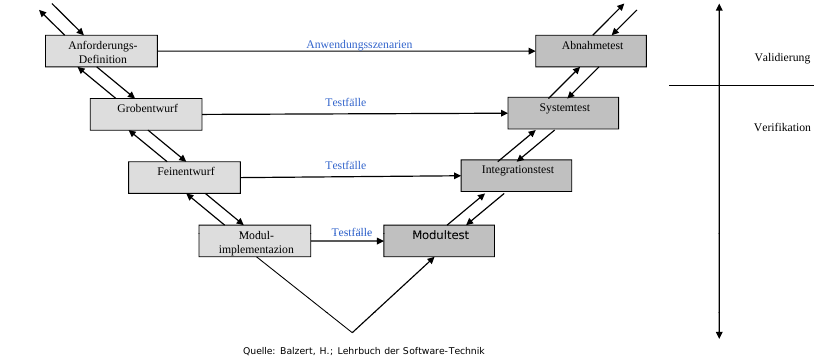
\includegraphics[width=0.8\linewidth]{./images/vmodell}
 \caption{V-Modell, Quelle: \cite{swscript}} %Universität Leipzig, Softwaretechnik}
 \label{fig:vmodell}
\end{figure}
Eine wichtige Rolle spielt die Qualitätssicherung, die das V-Modell sicher stellt. In diesem Modell sind die Verifikation und die Validation ein 
fester Bestandteil. Verifikation bedeutet, die Sicherstellung dass das entwickelte Produkt mit den Spezifikationen übereinstimmt.
Die Validation ist die Eignung des Produkts bezogen auf seinen Einsatzzweck. Durch die Sicherstellung beider Qualitätsmerkmale wird das Projekt 
erfolgreich zu seinem Ziel, die Antnennennachführung für Satelliten, geführt. Aus diesem Grund ist das V-Modell die richtie Vorangehensweise für 
dieses Projekt.
\newpar

\section{Zeitplan}
Bevor ein Projekt starten kann, ist wichtig  zu definieren, wie viel Zeit für die Durchführung zu Verfügung steht. Für diese Studienarbeit 
wird drei Studierenden einen Zeitrahmen von zwei Semerster zugeschrieben. Beginn der Studienarbeit ist der 14. Oktober 2015 und endet am 15. Juli 
2016. Für die Studierenden der Kurse TEN, TEK und TLE ist im Studenplan jeder Mittwoch von 14 Uhr bis 17.15 Uhr Studienarbeitszeit vorgesehen. Dies 
ist eine grobe Richtlinie für die Durchführung der Studienarbeit und kann nach Bedarf angepasst werden.
\newpar

\section{Anforderungsdefinition}
Inbetriebnahme einer quelloffenen, kostenfreien Software zur Antennennachführung für das Verfolgen von erdnahen Satelliten. Die zur 
Antennennachführung
benötigten Schnittstellen werden von der Hochschule zur Verfügung gestellt und sollen für diese Arbeit verwendet werden. Die Software soll die 
Satellitenposition mit Hilfe der Keplerelemente berechnen und ausgeben. Die Ausgabe soll grafisch erfolgen und anzeigen, wann
der gewählte Satellit verfügbar ist. Ist der gewählte Satellit verfügbar, soll die Antenne in die richtige Position nachgeführt werden. 
\newpar

\section{Arbeitspakete}
Arbeitspakete brechen das Projekt in einzelne Aufgaben runter und werden an einen 
zuständigen Mitarbeiter zugeteilt. Ein Arbeitspaket ist granular, das heißt es kann quantitativ und 
qualitativ von einem Mitarbeiter bearbeitet werden. Außerdem ist ein Arbeitspaket zeitlich begrenzt 
und dient der Projektfortschrittskontrolle. 
Daher ergibt sich ein detaillierter Projektablauf und ein Projektstrukturplan entsteht. In einem 
Projektstrukturplan sind alle im Projekt durchzuführenden Arbeiten aufgelistet und thematisch 
gegliedert. Für diese Projektarbeit ergibt sich folgender Projektstrukturplan 
\ref{fig:projektstruktur}:\\
\begin{figure}[h]
 \centering
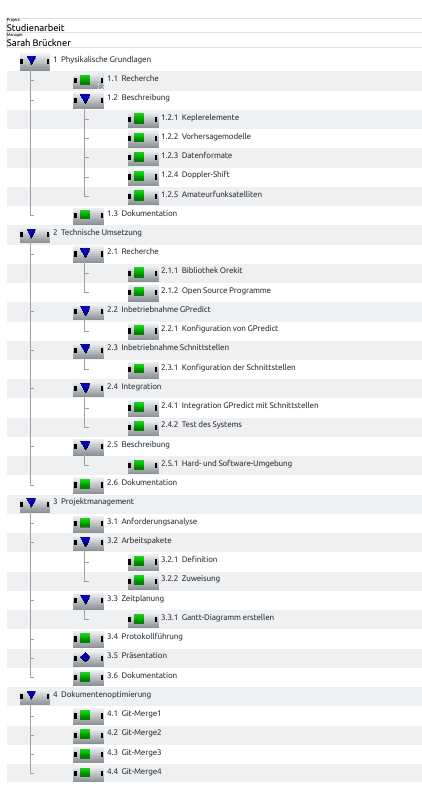
\includegraphics[width=0.5\linewidth]{./images/00tasks}
\caption{Projektstrukturplan}
 \label{fig:projektstruktur}
\end{figure}
\\
Die Studienarbeit ist in vier Themen aufgeteilt: Physikalische Grundlagen, Technische Umsetzung, 
Projektmanagement und Dokumentation. Fragen wie, ``Was ist unter den Keplerelemente zu 
verstehen und wie kann aus ihnen Azimut und Elevation bestimmt werden?'', müssen bei dem Arbeitspaket Physikalischer Hintergrund  beantwortet 
werden. Diese Beschreibung ist grundlegend zum Verständnis der zu in Betrieb nehmenden Software 
für die Satelliten Verfolgung und  Antennennachführung. Das Inbetriebnehmen der Software wird in der ``Technischen Umsetzung'' 
durchgeführt. Dabei muss im ersten Schritt eine geeignete Software validiert werden. Die 
Inbetriebnahme setzt auch das Wissen über die Hard- und Softwareumgebung voraus, welche zu 
verwenden ist. Es folgt die Konfiguration und Test der geeigneten Software mit den definierten 
Schnittstellen.
\newpar
Das Projektmanagement definiert die einzelnen Teilaufgaben und koordiniert diese in einem zeitlich 
festgelegten Rahmen um zu einem ergebnisorientierten Projektabschluss zu gelangen. Dabei ist auch 
das Erstellen einer Präsentation Teilaufgabe des Projektmanagements.
\newpar
Die Dokumentation dieser Studienarbeit beschreibt den gesamten Projektentwicklungsprozess. Dabei wurden die Themen nach den Arbeitspaketen 
aufgeteilt. Der zugewiesene Student des Arbeitspakets hat daher die Aufgabe, seine Erkenntnisse zu dokumentieren. Allgemein wurde sich 
auf das Drucksatzsystem zur Textformatierung \LaTeX geeinigt. Daher ist für die schriftliche Ausarbeitung dieser Studienarbeit eine 
fortlaufende Dokumentenoptimierung nötig. Um das Arbeiten von drei Studierenden an einem Dokument zu ermöglichen wird sich an dem freien 
Softwaretool ``Git'' zur verteilten Versionsverwaltung bedient. Je vier Termine zu einem ``Merge'' (engl., Zusammenführen) der 
aufgeteilten Ausarbeitungen werden zur Versionsverwaltung genutzt und dabei Änderungen von Formatierung diskutiert und zusätzlich 
Arbeitspaketfortschritte erörtert. 
\newpar
Durch das Aufgliedern des Projekts in einzelne Arbeitspakete wurden die Prozesse, Aktivitäten die durchzuführen sind, die Reihenfolge des 
Arbeitsablaufes durch die definierte Zeitvorgabe, die Ergebnisdefinition, die vorhandenen Ressourcen sowie die anzuwendenden Werkzeuge (\LaTeX und 
Git) definiert.  
In der folgenden Grafik \ref{fig:arbeitspaket} sind alle für die Studienarbeit benötigten 
Arbeitspakete mit Titel (Name), Verantwortlichem (Responisble), Zuweisung (Allocation) und 
Arbeitszeit (Estimate) aufgeführt.
\begin{figure}[h] 
 \centering
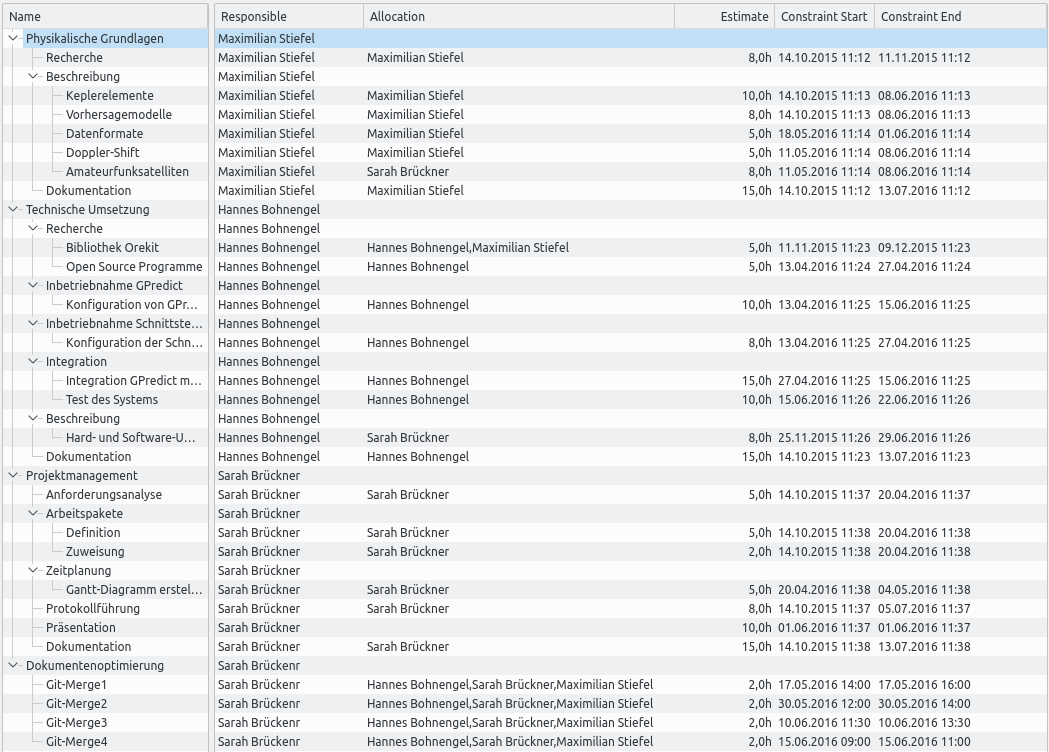
\includegraphics[width=1.0\linewidth]{./images/03task}
\caption{Arbeitspakete}
 \label{fig:arbeitspaket}
\end{figure}
\newpage

Der Arbeitspaketverantwortliche besitzt die Verantwortung für die Arbeitspaketdurchführung in 
Qualität, Zeit und Kosten. Dieser Steuert und hat die Kontrolle aller Arbeiten in seinem 
Arbeitspaket. Ebenso Koordiniert der Verantwortliche seine im Arbeitspaket beteiligten Mitarbeiter. 
Die Berichterstattung über den Status im Arbeitspaket folgt bei einem der ``Merges''.
\newpar

\section{Gantt-Diagramm}
Um die einzelnen Arbeitspakete koordinieren zu können werden aus diesen ein Gantt-Diagramm 
erstellt. Hier werden die einzuhaltenden Endtermine der einzelnen Arbeiten sowie die 
Parallelisierung von unabhängig zueinander liegenden Arbeiten geplant. Die Erstellung eines Gantt-Diagramms erfolgt mit dem Programm ``Plan'' zur 
Projektplanung und -verwaltung. 
\begin{figure}[h] 
 \centering
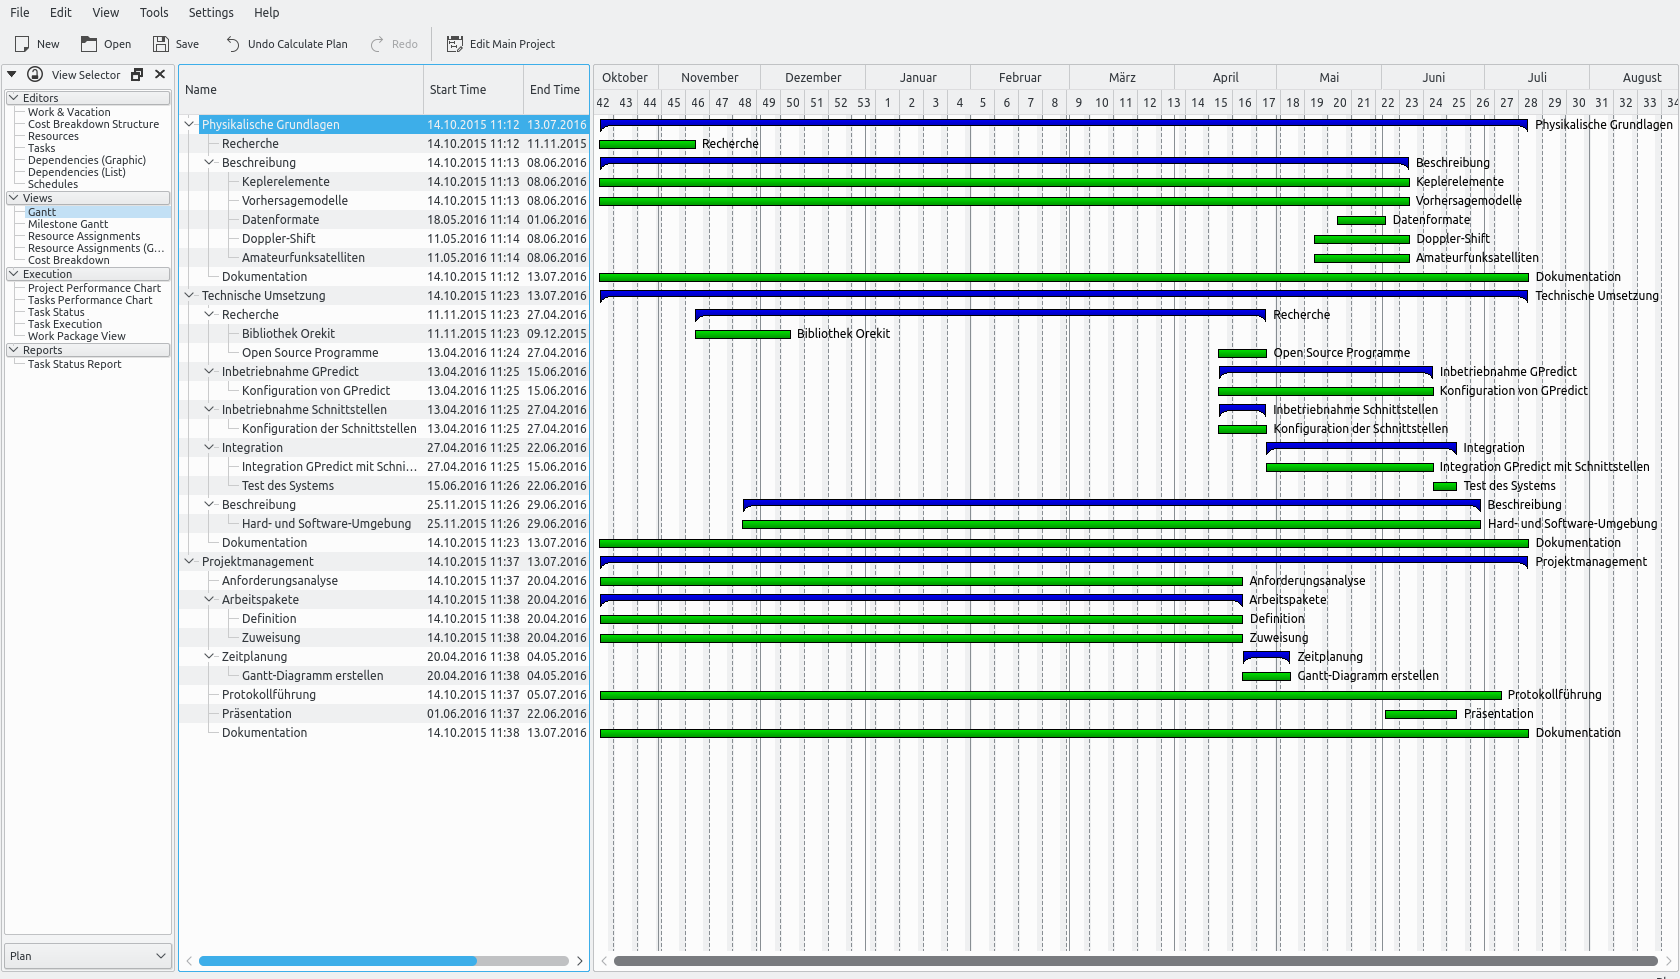
\includegraphics[width=1.0\linewidth]{./images/gantt}
\caption{Gantt-Diagramm}
 \label{fig:gantt}
\end{figure}
In der Grafik \ref{fig:gantt} wird die Parallelisierung der Arbeitspakete deutlich. Die drei Einheiten Physikalische Grundlagen, Technische Umsetzung 
und Projektmanagement können parallel bearbeitet werden. Begonnen wird mit einer umfassenden Recherche über die Keplerelemente und deren Berechnung. 
Parallel dazu kann über die  Realisierung der Software für die Satellitenverfolgung recherchiert werden. Die dadurch gewonnenen Erkenntnisse führen 
zu der Anforderungsdefinition. Analog zum V-Modell kann nun der nächste Schritt eingeleitet werden. Dieser entspricht in dieser Studienarbeit der 
Inbetriebnahme von der Software ``GPredict''. Zu diesem Arbeitspaket gehören die Aufgaben Konfiguration der Software und Konfiguration der 
Schnittstellen. Darüber hinaus muss sich der Verantwortliche umfassend mit der Software auseinander setzen um im nächsten Schritt die Integration 
beider Komponenten, Software und Hardware, durchzuführen. Ist eine funktionsfähige Kommunikation beider Komponenten bereitgestellt, können Tests, wie 
das Verfolgen von Satelliten, geprüft werden. Bei den Tests wird unterschieden in Modultest, das Testen der einzelnen Komponenten auf ihre 
Funktionsfähigkeit, Integrationstest, Kommunikationsfähigkeit der Software mit der Hardware und Systemtest, das Verfolgen von Satelliten und 
Antennennachführung. Alle Erkenntnisse die in den Arbeitspaketen gewonnen wurden müssen dokumentiert werden. Daraus schließt sich das letzte 
Arbeitspaket, die Dokumentation und die damit einhergehende Dokumentenoptimierung.